\documentclass[a4paper]{sbgames}               % final
%\usepackage[scaled=.92]{helvet}
\usepackage{times}
\usepackage{graphicx}

%% use this for zero \parindent and non-zero \parskip, intelligently.
\usepackage{parskip}

%% the 'caption' package provides a nicer-looking replacement
\usepackage[labelfont=bf,textfont=it]{caption}

\usepackage{listings}
\usepackage{color}

\definecolor{dkgreen}{rgb}{0,0.6,0}
\definecolor{gray}{rgb}{0.5,0.5,0.5}
\definecolor{mauve}{rgb}{0.58,0,0.82}

\lstset{frame=tb,
  language=C,
  aboveskip=3mm,
  belowskip=3mm,
  showstringspaces=false,
  columns=flexible,
  basicstyle={\small\ttfamily},
  numbers=none,
  numberstyle=\tiny\color{gray},
  keywordstyle=\color{blue},
  commentstyle=\color{dkgreen},
  stringstyle=\color{mauve},
  breaklines=true,
  breakatwhitespace=true,
  tabsize=3
}

\usepackage{url}
\usepackage[utf8]{inputenc}
%% Paper title.
\title{Computer Graphics}

%% Author and Affiliation (multiple authors). Use: and between authors

\author{Alexandre Tolstenko Nogueira\\InfiniBrains\\tolstenko@infinibrains.com.br 
%        \and Name2 B. Surname2\\ Name3 C. Surname3\\ ZZZZ University
%        \and Name4 D. Surname4\\ Farwest Research Center 
}
\contactinfo{\{name1,name3\}@xxx.yyyy.yyy \\
             *name2@zzzz.vvvv.vvv
}
%% Keywords that describe your work.
\keywords{Real-time Strategy, Relief Mapping, Shortest Path Algorithm, First Person Shooting}

%% Start of the paper
% Attention: As you need to insert EPS images in Postscript, 
% you need to insert PDF images into PDFs. 
% In the text, extensions cancbe omitted (latex use .eps, pdflatex get .pdf) 
% To convert them: epstopdf myimage.eps
\begin{document}

%\teaser{
%  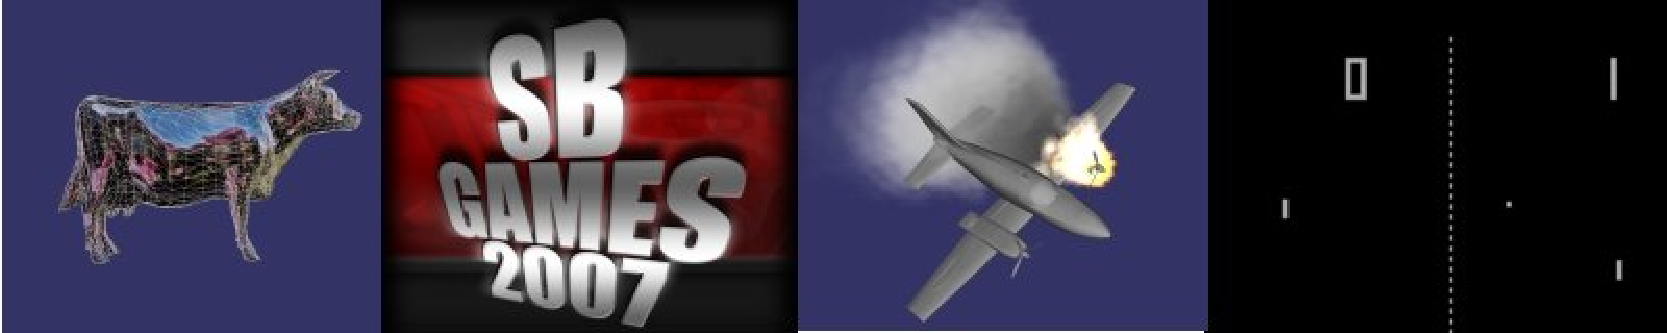
\includegraphics[width=\linewidth]{sample.pdf}
%  \caption{Optional image}
%}

%% The ``\maketitle'' command must be the first command after the
%% ``\begin{document}'' command. It prepares and prints the title block.

\maketitle

%% Abstract section.

%\begin{abstract}
%  This meta-paper describes the model to be used in papers and posters
%  for SBGames. In the subsection Author's contact, make reference to
%  the same symbol used in the affiliation.
%\end{abstract}

%% The ``\keywordlist'' command prints out the keywords.
%\keywordlist
%\contactlist

\section{Atividade Aula 4 - Fundamentos de Processamento Gráfico}

\subsection*{Questionário}

\textbf{1)Continuar a implementação do programa de processamento de imagens da aula anterior: implementar o filtro passa-alta e mais dois métodos de detecção de bordas (você pode escolher). Devem ser entregues em um arquivo PDF: o programa fonte e um exemplo de imagem processada (incluir imagem original e imagem resultante) para
cada um dos três métodos implementados}

Todas as implementações estão disponíveis publicamente no github da game engine que estou desenvolvendo \cite{Tolstenko2018}.

A diferença básica entre o filtro de Sobel e o de kirsch é que o filtro de segundo consegue capturar melhor as nuances de gradientes diagonais.

Apply Mask
\begin{lstlisting}
float EditorGUI::ApplyMask(unsigned char *input, int width, int height, int line, int column, float *mask, int maskWidth, int maskHeight, int bytesPerChannels, int numberOfChannels) {
  // TODO: handle borders
  if (column >= width - maskWidth/2 + 1 || column <= maskWidth/2 - 1 || line >= height - maskHeight/2 + 1 || line <= maskHeight/2 - 1)
    return 0;

  float ret = 0;
  for (int y = -maskHeight/2; y <= maskHeight/2; y++) {
    for (int x = -maskWidth/2; x <= maskWidth/2; x++) {
      int pos = ((line+y) * width + column+x) * numberOfChannels * bytesPerChannels;
      float color = 0;
      for (auto i = 0; i < numberOfChannels - 1; i++)
        color += input[pos + i];
      color /= numberOfChannels - 1; // the average of all channels
      color *= mask[x + maskWidth/2 + (y + maskHeight/2) * maskWidth]; // apply mask
      ret += color; // accumulate the value
    }
  }

  return ret;
}
\end{lstlisting}

\pagebreak
Laplace
\begin{lstlisting}
void EditorGUI::Laplace(unsigned char * input, unsigned char * output, int width, int height, int bytesPerChannels, int numberOfChannels)
{
  if(numberOfChannels!=4 || bytesPerChannels!=1)
    throw NotImplementedException();

  float laplace[] = {-1,-1,-1,
                          -1, 8,-1,
                          -1,-1,-1};

  for(int line =0;line<height;line++){
    for(int column =0;column<width;column++){
      int pos = (line * width + column) * numberOfChannels * bytesPerChannels;

      auto value = ApplyMask(input,width,height,line,column,laplace,3,3);
      auto color = (unsigned char) MIN(MAX(value,0),255);

      output[pos]  =color;
      output[pos+1]=color;
      output[pos+2]=color;
      output[pos+3]=255;
    }
  }
}
\end{lstlisting}

\pagebreak
Sobel
\begin{lstlisting}
void EditorGUI::Sobel(unsigned char *input, unsigned char *output, int width, int height, int bytesPerChannels, int numberOfChannels)
{
  if(numberOfChannels!=4 || bytesPerChannels!=1)
    throw NotImplementedException();

  float vert[] = {-1,0,+1,
                       -2,0,2,
                       -1,0,1};
  float hor[] = { 1, 2, 1,
                       0, 0, 0,
                      -1,-2,-1};

  for(int line =0;line<height;line++){
    for(int column =0;column<width;column++){
      int pos = (line * width + column) * numberOfChannels * bytesPerChannels;

      auto vertvalue = ApplyMask(input,width,height,line,column,vert,3,3);
      auto horivalue = ApplyMask(input,width,height,line,column,hor,3,3);

      auto color = (unsigned char) MIN(MAX(sqrt(vertvalue*vertvalue + horivalue*horivalue),0),255);

      output[pos]  =color;
      output[pos+1]=color;
      output[pos+2]=color;
      output[pos+3]=255;
    }
  }
}
\end{lstlisting}

\pagebreak
Kirsch
\begin{lstlisting}[basicstyle=\scriptsize\ttfamily,]
void EditorGUI::Kirsch(unsigned char *input, unsigned char *output, int width, int height, int bytesPerChannels, int numberOfChannels)
{
  if(numberOfChannels!=4 || bytesPerChannels!=1)
    throw NotImplementedException();

  float v1[] = { 5,  5,  5,
                     -3,  0, -3,
                     -3, -3, -3};
  float v2[] = { 5,  5, -3,
                      5,  0, -3,
                     -3, -3, -3};
  float v3[] = { 5, -3, -3,
                      5,  0, -3,
                      5, -3, -3};
  float v4[] = {-3, -3, -3,
                      5,  0, -3,
                      5,  5, -3};
  float v5[] = {-3, -3, -3,
                     -3,  0, -3,
                      5,  5,  5};
  float v6[] = {-3, -3, -3,
                     -3,  0,  5,
                     -3,  5,  5};
  float v7[] = {-3, -3,  5,
                     -3,  0,  5,
                     -3, -3,  5};
  float v8[] = {-3,  5,  5,
                     -3,  0,  5,
                     -3, -3, -3};

  for(int line =0;line<height;line++){
    for(int column =0;column<width;column++){
      int pos = (line * width + column) * numberOfChannels * bytesPerChannels;

      auto r1 = ApplyMask(input,width,height,line,column,v1,3,3);
      auto r2 = ApplyMask(input,width,height,line,column,v2,3,3);
      auto r3 = ApplyMask(input,width,height,line,column,v3,3,3);
      auto r4 = ApplyMask(input,width,height,line,column,v4,3,3);
      auto r5 = ApplyMask(input,width,height,line,column,v5,3,3);
      auto r6 = ApplyMask(input,width,height,line,column,v6,3,3);
      auto r7 = ApplyMask(input,width,height,line,column,v7,3,3);
      auto r8 = ApplyMask(input,width,height,line,column,v8,3,3);

      // 765 == 3*255 -> this is used to clamp the maximum pixel value properly
      auto max = MIN(MAX(MAX(MAX(MAX(r1,r2),MAX(r3,r4)), MAX(MAX(r5,r6),MAX(r7,r8))),0),765)/3;
      auto color = (unsigned char) max;

      output[pos]  =color;
      output[pos+1]=color;
      output[pos+2]=color;
      output[pos+3]=255;
    }
  }
}
\end{lstlisting}
\pagebreak

\begin{figure} [h!]
  \centering 
  \includegraphics[width=0.95\linewidth]{imgs/highpass}
 \caption{Quadrante superior esquerdo: imagem original; superior direito: aplicação do filtro laplaciano; inferior esquerdo: aplicação do filtro de sobel; inferior direito: aplicação do filtro de kirsch.} 
 \label{fig:burstgoogle} 
\end{figure}

\pagebreak

\textbf{2) Encontre as transformações de visualização de um sistema cuja camera está posicionada na posição $(3,3,3)$, o plano de projeção é definido pelo ponto $(1,1,1)$ e pelo vetor $(-1,-1,-1)$ e o espaço de imagem é definido por um quadrado de lado $20$ centrado na origem do plano de projeção.}

\textbf{3) Considere este mesmo modelo de camera e ainda $s_x = s_y = 1$, $u_c = 600$ e $v_c = 400$ e encontre as coordenadas da projeção do ponto $(0,0.5,0.5) \in R^3$}

\textbf{4) Descreva como fica a transformação projetiva com mais de um ponto de fuga.}

Infelizmente não consegui terminar, mas encontrei um excelente material:

{\tiny{\url{https://www.scratchapixel.com/lessons/3d-basic-rendering/computing-pixel-coordinates-of-3d-point/mathematics-computing-2d-coordinates-of-3d-points}}}

\bibliographystyle{sbgames}
\bibliography{template}
\end{document}